\documentclass[a4]{article}
%\usepackage{czech}
\usepackage{graphicx}
\usepackage[utf8]{inputenc}   % pro unicode UTF-8
\usepackage{booktabs}
\usepackage{hyperref}
%#\usepackage{qtree}
%\usepackage{graphviz}
\usepackage{authblk}
%\usepackage{tikz-dependency}
\usepackage[ampersand]{easylist}

%\usepackage{verse}

\def\furl#1{\footnote{\url{#1}}}


\begin{document}

\title{Neuronový strojový překlad z němčiny do češtiny}

\author{Dominik Macháček}
\affil{
%Saarland University, Saarbrücken, Germany,
dominik.machacek@matfyz.cz
}

\date{\today}

%\pacs{PACS numbers go here. These are classification codes for your  research. See {\tt http://publish.aps.org/PACS/} for more info.}
\maketitle

%\begin{abstract}
%TODO: An abstract is a great convenience for the reader and is required by all journals.
%\end{abstract}


\section{Úvod}

V tomto článku shrnujeme experimenty trénování neuronového strojového
překladu z~němčiny do češtiny s~použitím OpenNMT.

\section{Předchozí práce zabývající se překladem z~němčiny do češtiny}

\subsection{Zeman: frázový překlad pro WMT13}

Dosud nejlepší strojový překlad z~němčiny do češtiny vytvořil Dan Zeman
v~roce 2014. Systém je popsán v~článku \cite{zeman}.

Jedná se o frázový překlad s~použitím systému Moses. Pro trénování autor
použil paralelní korpusy Europarl a News Commentary ve verzích, jaké byly
k~dispozici jako trénovací data pro
WMT13\furl{http://www.statmt.org/wmt13/translation-task.html}. Pro vývoj
sloužila sada překladů novinových článků News Commentary 2011, pro testování
News Commentary 2013.

Ve fázi preprocessingu byla data tokenizována, zvláštní znaky byly
normalizovány nebo odstraněny. Následně byly normalizována reprezentace
uvozovek a byl aplikován truecasing.

%Například slovo {\it Nationalessen} je
%složeno ze slov {\it National} (národní) a {\it Essen} (jídlo). Samo o sobě
%ve slovníku být nemusí, ale každé z~jeho kořenů ano. Proto 
%

Dále se autor snažil vyřešit problém s~německými složenými slovy, která
zvyšují počet neznámých slov. K tomu použil nástroj
Morfessor\cite{morfessor}. Text je před překládáním rozdělen na morfémy,
poté přeložen a poté opět složen do celých slov.

TODO: jak to vlastně je? A co lemmatizace?

Pro přehledné porovnání s~ostatními překladatelskými systémy je výsledek
nahrán na \url{matrix.statmt.org}.

\subsection{Tlustý: Využí hrubé reprezentace slov ve strojovém
překladu do češtiny}

V roce 2016 vznikla diplomová práce Marka Tlustého \cite{tlusty}, ve které se autor
zabývá dělením německých a maďarských slov na kratší části podle jejich
morfologického významu. Dělí se tedy např. na morfémy nebo jednotlivé kořeny
složených slov. To má sloužit ke snížení podílu neznámých slov v~testovací
množině oproti trénovací a ke zlepšení frázového překladu. 

Autor experimentoval s~několika strategiemi a existujícími nástroji, téměř
všechny vykázaly zlepšení podle metrik BLEU a METEOR oproti systémům bez
hrubé reprezentace.  Překlad byl realizován sysémem Moses. Autor použil
korpus Europarl\cite{europarl}, který sám rozdělil na trénovací, testovací a vývojovou
část. 

V~práci není srovnání s~předchozím překladem Dana Zemana, ani v~ní nejsou
vloženy výsledné natrénované modely. Rovněž práce neobsahuje podrobný manuál, jak
zreplikovat její nejlepší výsledky.

Neuronový strojový překlad se v~práci vůbec nezmiňuje. 
U něj se rovněž používá hrubá reprezentace slov, nejčastěji
tzv. byte pair encoding, u něhož se dělí slova na podslova podle absolutní četnosti jejich
částí. Na morfologický význam vzniklých podslov se nebere zřetel. Toto je
jiná strategie než u frázového překladu a v~práci se neuvádí. 

%To, že strategie pro hrubou reprezentaci slov pro frázový překlad budou vykazovat dobré
%výsledky i pro neuronový překlad, není zřejmé.


\section{Data}

Pro trénování našeho systému pro strojový překlad jsme postupně vyzkoušeli tři množiny
paralelních německo-českých dat: Europarl, OpenSubtitles a spojení Europarlu
a OpenSubtitles. Velikost korpusů udává tabulka \ref{tab:data}.

\begin{table}[ht]
\begin{verbatim}
trénovací data            |  počet vět
======================================
Europarl                  |    555 399
pročištěný_Europarl       |    555 022
OpenSubtitles             |  9 344 614
pročištěné_OpenSubtitles  |  8 212 213
Europarl+OpenSubtitles    |  8 767 235
                          
dev: News 11              |      3 000
test: News 13             |      3 005
\end{verbatim}
\caption{Velikost všech částí použitých dat}
\label{tab:data}
\end{table}


Pro vývojov a testování jsme použili stejná data jako v~baselinovém systému
Dana Zemana.

\subsection{Příprava dat}

\subsubsection{Předzpracování dat}

Všechna data jsme předzpracovali stejným postupem jako v~baselinovém
systému. Data byla tokenizována, zvláštní znaky byly
normalizovány nebo odstraněny. Následně byly normalizována reprezentace
uvozovek. K~tomu jsme použili nástroje ze systému Moses\cite{moses}.

Truecasing ani lowercasing jsme na rozdíl od frázového překladu neaplikovali.


\subsubsection{Pročištění Europarlu}

Zevrubnou analýzou Europarlu jsme zjistili, že v~česko-německé části jsou některé
věty špatně přeložené či špatně anotované. Příkladem jsou věty v~tabulce
\ref{tab:europarl}. Některé věty jsou ve skutečnosti v~angličtině či v~jiném
jazyce, ale jsou označeny jako české. Některé věty zřejmě pochází
z~projevu v~určitém jazyce, do kterého řečník vložil latinskou, chorvatskou
či obdobnou větu v~jiném jazyce, než v~jakém pronášel projev. V~korpusu
tyto věty nepřekládají. 

Takovéto věty by mohly negativně ovlivnit kvalitu překladu. Proto jsme se
rozhodli je odfiltrovat. K~tomu jsme použili
nástroj pro detekci jazyka {\tt langdetect}\cite{langdetect} a několik
dalších pravidel, která jsme odpozorovali na části korpusu.

\begin{table}[ht]
\begin{verbatim}
cs: Izvolite, prosim!
de: Izvolite, prosim!

cs: (Die Sitzung wird um 9.00 eröffnet.)
de: (Die Sitzung wird um 00 eröffnet.)

cs: Citizens should be able to hold law-makers accountable.
de: Die Bürger müssen in der Lage sein, von den Gesetzgebern Rechenschaft zu
verlangen.

cs: (La seduta è tolta alle 22.20)
de: (Die Sitzung wird um 20 Uhr geschlossen.)

cs: (
de: (

cs: Caveant consules!
de: Caveant consules!
\end{verbatim}
\caption{Příklady nekvalitních vět v~Europarlu.}
\label{tab:europarl}
\end{table}

\subsubsection{Pročištění titulků}

Korpus OpenSubtitles je velmi rozsáhlý, ale není považován za kvalitní
zdroj pro neuronový strojový překlad, protože mnohé věty, které obsahuje,
jsou velmi krátké nebo nejsou přesně zarovnány. Takovéto věty jsme se
použili odfiltrovat jednoduchým pravidlem. Krátké věty jsme se snažili
odfiltrovat tak, že jsme zahodili ty věty, které v~češtině i v~němčině měly
méně než 4 slova. Špatně zarovnané věty jsme se snažili odfiltrovat tak, že
jsme zahodily ty věty, u kterých rozdíl počtu slov byl větší než 16. Tato
pravidla zřejmě nejsou optimální, ale použili jsme je alespoň jako
startovací parametry.

Rovněž jsme zjistili, že v~některých českých větách se vyskytují slova jako
{\it skvěIý}, ve kterých je znak {\it I} místo {\it l}. To jsme se snažili
napravit regulárním výrazem.

\subsection{Hrubá reprezentace slov: Morfessor a BPE}

Následně jsme se snažili vyřešit problém s~bohatými slovníky rozdělením
slov na podčásti. Nejdříve jsme zopakovali postup Dana Zemana a použili
nástroj Morfessor\cite{morfessor}, čímž se snížil počet slov na méně než
desetinu, viz tabulka \ref{tab:morf}.


\begin{table}[ht]
\begin{verbatim}
data                       |  Training set unique 1-grams
========================================================
de, tokenizovaný Europarl  |  191741        (100  %)
de, Morfessor, Europarl    |   18008        (9.4  %)
--------------------------------------------------------
cs, tokenizovaný Europarl  |  183227        (100  %)
cs, Morfessor, Europarl    |   16477        (8.9  %)
\end{verbatim}
\caption{Velikost slovníku trénovacích dat před a po použití Morfessoru}
\label{tab:morf}
\end{table}



Poté jsme ještě vyzkoušeli
byte-pair-encoding s~různými počty slov, a to 7500, 30000, 50000 a 80000.


\section{Automatická evaluace}

Pro evaluaci všech modelů používáme skript pro BLEU skóre \texttt{multi-bleu.perl} ze systému
Moses\cite{moses}. Výsledky skriptu záleží na námi použité tokenizaci, není
proto vhodné naše BLEU skóre porovnávat
s~překlady stejných testovacích dat jinými systémy s~jinými tokenizátory.

Pro porování s~baselinovým frázovým překladem Dana Zemana jsme jeho
testovací data tokenizovali naším tokenizátorem a použili náš evaluační
skript. Jeho BLEU skóre je 13.99.

Před použitím skriptu naše přeložená data postprocesujeme, hrubou reprezentaci
slov převádíme na původní.

\section{Trénování modelů s~OpenNMT}

Pro natrénování neuronového překladu jsme se rozhodli použít systém
OpenNMT\cite{opennmt}. 
%Zde shrneme několik problémů s~tímto frameworkem, na které jsme narazili:
%
%-- instalace: torch a LuaJit vs Lua5.2
%
%-- padá to na nedostatek paměti
%
%-- padá to bez chybové hlášky
%
%-- dokumentace se rychle mění
%
%-- dokumentace instalace v~jednu chvíli nebyla úplná
%
%-- ve kterém luarocks se mají nainstalovat knihovny? ve kterém source?
%
%TODO
%



\subsection{Trénování s~OpenNMT-py a Morfessorem}

Pro první experimenty s~trénováním jsme použili OpenNMT-py a Europarl s~dělení slov
podle Morfessoru. Modely jsme průběžně vyhodnocovali podle
BLEU skóre, nejlepší skóre na testovacím vstupu bylo 4.74.

Na základě těchto experimentů a faktu, že OpenNMT-py nedokáže paralelní
trénink na více grafických kartách, jsme se rozhodli pro ostatní
experimenty používat OpenNMT-Lua.

\subsection{Trénování s~BPE a OpenNMT-Lua}



\subsubsection{Popis konfigurací}

Následující konfi

-- defaultní konfigurace
	-- validation metric: perplexity
-- rychlost trénování



\begin{verbatim}
label                      |  data           |  BPE   |  batch  |  layers  |  GPU  |
====================================================================================
europarl-1gpu30000-1       |  Europarl       |  30k   |  64     |  2       |  1    |
europarl-1gpu30000-3       |  navazuje_na-1  |  30k   |  1      |  2       |  1    |
europarl-1gpu30000-4       |  navazuje_na-1  |  30k   |  64     |  2       |  1    |
europarl-1gpu30000-5       |  navazuje_na-4  |  30k   |  64     |  2       |  1    |
europarl-1gpu30000-6       |  navazuje_na-4  |  30k   |  32     |  2       |  1    |
europarl-1gpu50000-1       |  Europarl       |  50k   |  64     |  2       |  1    |
europarl-1gpu7500-1        |  Europarl       |  7500  |  64     |  2       |  1    |
europarl-1gpu80000-1       |  Europarl       |  80k   |  64     |  2       |  1    |
osub-europarl-1gpu30000-1  |  OpenSub+EuP    |  30k   |  64     |  2       |  1    |
osub-europarl-1gpu50000-1  |  OpenSub+EuP    |  50k   |  64     |  2       |  1    |
osub-europarl-1gpu80000-1  |  OpenSub+EuP    |  80k   |  64     |  2       |  1    |
osub-europarl50000-2       |  OpenSub+EuP    |  50k   |  64     |  3       |  4    |
baseline-ZEMAN             |  Eup+NewsComm   |  -     |  -      |  -       |  -    |
 
label                      |  rychlost_epochy       |  epochs     |  best_test_BLEU
====================================================================================
europarl-1gpu30000-1       |  2min_(save_every50)   |  1-15       |  11.50
europarl-1gpu30000-3       |  1h_(save_every2000)   |  15-21-30?  |  4.95
europarl-1gpu30000-4       |  7m_(save_every2000)   |  15-30      |  11.55
europarl-1gpu30000-5       |  3m_(save_every2000)   |  30-90      |  11.69
europarl-1gpu30000-6       |  00m_(save_every2000)  |  30-90      |  11.66
europarl-1gpu50000-1       |  7min_(save_every50)   |  1-15       |  11.27
europarl-1gpu7500-1        |  4min_(save_every50)   |  1-15       |  10.28
europarl-1gpu80000-1       |  90min_(save_every50)  |  1-15       |  10.89
osub-europarl-1gpu30000-1  |  0h20m_(save_every50)  |  1-14-15?   |  14.03
osub-europarl-1gpu50000-1  |  6h24m_(save_every50)  |  1-11-15?   |  13.76
osub-europarl-1gpu80000-1  |  1h47m_(save_every50)  |  1-14-15?   |  14.00
osub-europarl50000-2       |  h13m_(save_every500)  |  1-20       |  14.91
baseline-ZEMAN             |  -                     |  -          |  13.99
\end{verbatim}

%TODO: z logů můžeme vyčíst čas, který byl potřeba na ukládání všech checkpointů
%time spent on checkpoint saving
%data | iterations | save-every | batch | time-for-checkpoint-save | checkpoint-size


\subsubsection{Průběh trénování}

\ref{fig:europarl}

\ref{fig:osub}

\begin{figure}[h]
\centering
  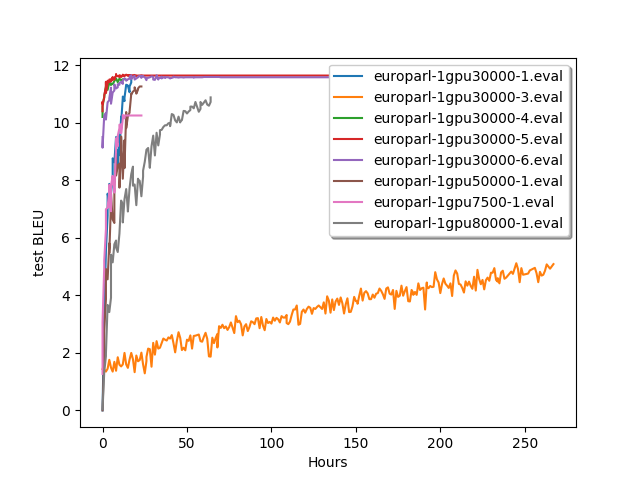
\includegraphics[width=1.3\linewidth]{europarl_test.png}
    \caption{BLEU skóre na testovací množině. Trénováno na Europarlu
	s~různými BPE.}
  \label{fig:europarl}
\end{figure}


\begin{figure}[h]
\centering
  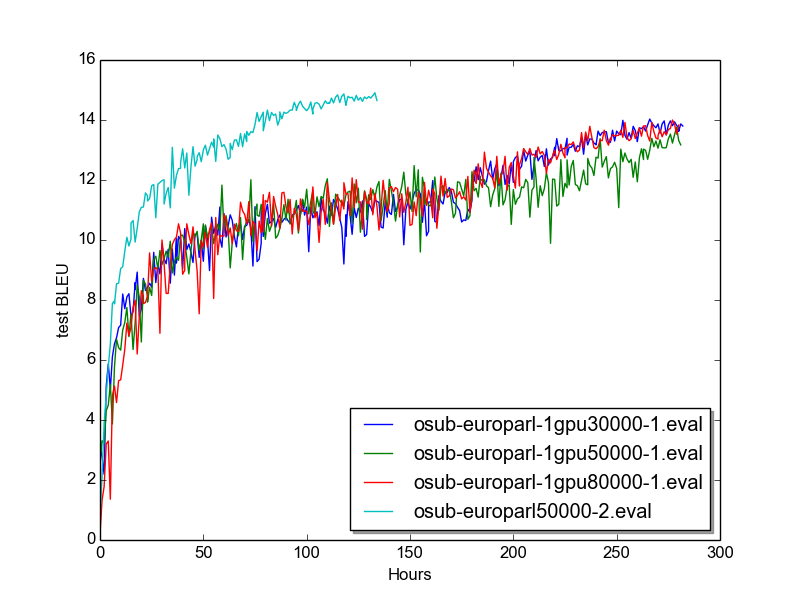
\includegraphics[width=1.3\linewidth]{osub_europarl_test.png}
    \caption{BLEU skóre na testovací množině. Trénováno na Europarlu
	s~různými BPE.}
  \label{fig:osub}
\end{figure}



\section{Analýza nejlepšího překladu}

\section{Závěr}


\begin{thebibliography}{99}



\bibitem{zeman}
 Ondřej Bojar, Daniel Zeman: {\sl Czech Machine Translation in the project
 CzechMATE}. Publikováno v~{\sl The Prague Bulletin of Mathematical
 Linguistics}, číslo 101., duben 2014, strany 71–96.

\bibitem{morfessor}
	Mathias Creutz, Krista Lagus: {\sl Unsupervised models for morpheme
	segmentation and
	morphology learning}. ACM Transactions on Speech and Language Processing
	(TLSP), 4(1)(3),
	2007. URL \url{http://dl.acm.org/citation.cfm?id=1187418}.

\bibitem{tlusty}
 Bc. Marek Tlustý: {\sl  Využí hrubé reprezentace slov ve strojovém
překladu do češtiny}. Diplomová práce. Praha, 2016.
% \url{https://github.com/Gldkslfmsd/sekacek}

\bibitem{moses}
 P. Koehn: Moses. TODO 



\bibitem{langdetect}
 Michal Danilák: {\sl langdetect: Port of Google's language-detection library to
 Python.}
 \url{https://github.com/Mimino666/langdetect}
% \url{https://github.com/Gldkslfmsd/sekacek}

\bibitem{opennmt}
 OpenNMT. \url{http://opennmt.net/about/}. TODO





\end{thebibliography}





\end{document}


